% Generated by code/scripts/report_figures.py at 2026-11-16T12:31:35Z; do not edit.
% Inputs: artifacts/cluster/runs/bench4-20261110T103706Z-1535991
\begin{figure}[t]
\centering
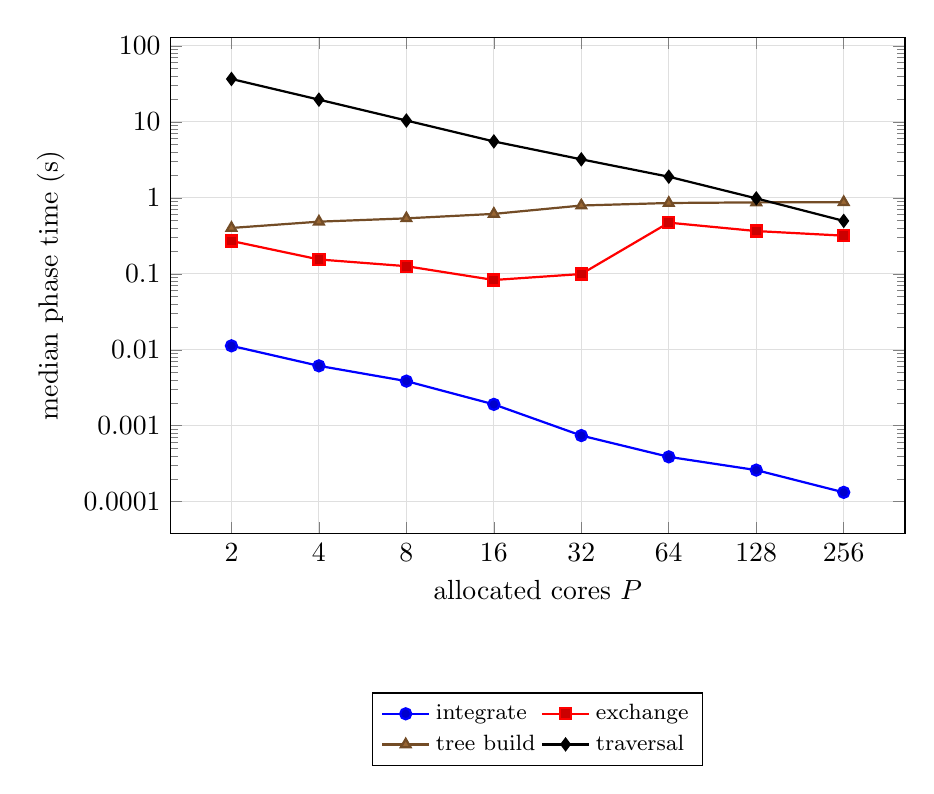
\begin{tikzpicture}
\begin{axis}[width=0.9\columnwidth, height=0.65\columnwidth, xlabel={allocated cores $P$}, ylabel={median phase time (s)}, xmode=log, log basis x=2, log ticks with fixed point, ymode=log, ytick={0.0001,0.001,0.01,0.1,1,10,100}, legend style={at={(0.5,-0.32)}, anchor=north, legend columns=2, font=\footnotesize}, legend cell align=left, grid=major, grid style={gray!25}]
\addplot+[mark=*, thick] coordinates {(2,0.01127) (4,0.006145) (8,0.003869) (16,0.001913) (32,0.000743) (64,0.00039) (128,0.000261) (256,0.000133)};
\addlegendentry{integrate}
\addplot+[mark=square*, thick] coordinates {(2,0.2704) (4,0.1544) (8,0.1259) (16,0.08286) (32,0.09932) (64,0.4707) (128,0.3651) (256,0.3174)};
\addlegendentry{exchange}
\addplot+[mark=triangle*, thick] coordinates {(2,0.401) (4,0.4853) (8,0.5365) (16,0.6143) (32,0.7914) (64,0.8544) (128,0.8703) (256,0.8755)};
\addlegendentry{tree build}
\addplot+[mark=diamond*, thick] coordinates {(2,36.61) (4,19.58) (8,10.4) (16,5.518) (32,3.207) (64,1.894) (128,0.9825) (256,0.4965)};
\addlegendentry{traversal}
\end{axis}
\end{tikzpicture}
\caption{Phase times of the strong-scaling runs with $T=1$. Each phase is the maximum over ranks, so the phases need not sum to the wall time; zero values are omitted from the log axis. Vanda job 1535991: 64 of 72 cores on each of four Platinum 8452Y nodes (CN-047, CN-061, CN-064, CN-065), 3 interleaved repetitions.}
\label{fig:b4-phases}
\end{figure}
